\documentclass[a4paper,11pt]{article}
\usepackage[utf8]{inputenc}
\usepackage{amsmath}
\usepackage{amsfonts}
\usepackage{amssymb}
\usepackage{graphicx}
\usepackage{braket}
\usepackage{listings}

\numberwithin{equation}{section}
\renewcommand\thesubsection{\alph{subsection}}
\newcommand{\bvp}[1]{\mathbf{#1}'}
\newcommand{\bv}[1]{\mathbf{#1}}

\lstset{breaklines=true}

%opening
\title{Computational Biophysics HW3}
\author{Vince Baker}

\begin{document}

\maketitle

\section{Q1}
For algorithms that attempt to minimize the starting potential energy through a method such as steepest descent, the temperature does not have an effect.
The gradient of the potential energy is a function of position only.\\
One could also search for an energy minimum by running the simulation with some initial temperature and letting the temperature approach zero during the simulation (annealing).
The system temperature sets the intensity of the thermal fluctuations that allow the system to cross local minima.
As the temperature approaches zero the system should settle towards the ground state, or at least a local minimum energy state.\\

\section{Q2}
i) The first and second peaks in the pair correlation function of a liquid are the nearest-neighbor and second-neighbor shells. \\
ii) The pair correlation function is normalized by the expected pair correlation function for an unordered system (ideal gas) of the same density.
The actual pair correlation function should approach 1 as $r \rightarrow \infty$ since we don't expect to see order at extremely long scales.
In molecular dynamics simulations using periodic boundary conditions the pair correlation function should not be calculated on length scales longer than the cell size, as PBCs impose nonphysical periodicity at those length scales.

\section{Q3}
See attached MATLAB script for code. The x-y positions  and remaining error at each step are:\\
\begin{tabular}{l c | r}
    X & Y & Error \\
    5.0000 &   4.0000 &  57.0000\\
    2.0915 &  -0.6536 &   5.2288\\
    0.4587 &   0.3669 &   0.4796\\
    0.1919 &  -0.0600 &   0.0440\\
    0.0421 &   0.0337 &   0.0040\\
    0.0176 &  -0.0055 &   0.0004\\
    0.0039 &   0.0031 &   0.0000\\
    0.0016 &  -0.0005 &   0.0000\\
    0.0004 &   0.0003 &   0.0000 
\end{tabular}

\section{P1}
The coordination function is close to 6 at the highest density, showing a hexagonal-type structure. 
At the lower densities the material is less ordered, so the nearest-neighbor cage does not have the same regualr packing.
This is reflected in the lower coordination numbers.\\
\begin{figure}[h]
 \caption{Effect of density upon coordination number}
 \centering
   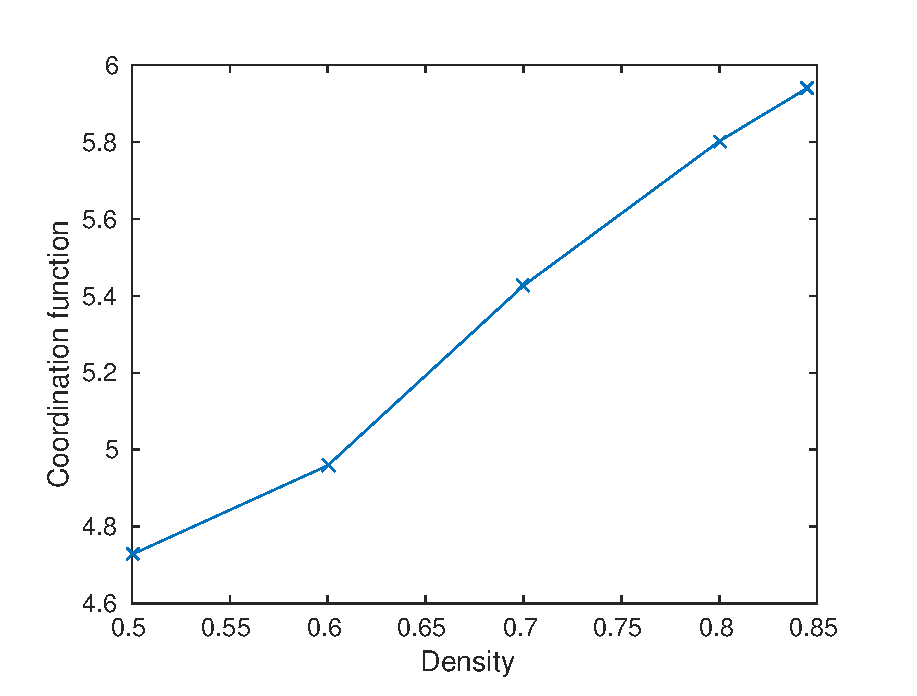
\includegraphics[width=\textwidth]{p1}
\end{figure}

\section{P2}
The coordination number for the 3-dimensional case is 11.74, very close to the expected coordination number of 12 for an FCC lattice.
\begin{figure}[h]
 \caption{Pair coorelation function for $\rho=0.845$ in three dimensions}
 \centering
 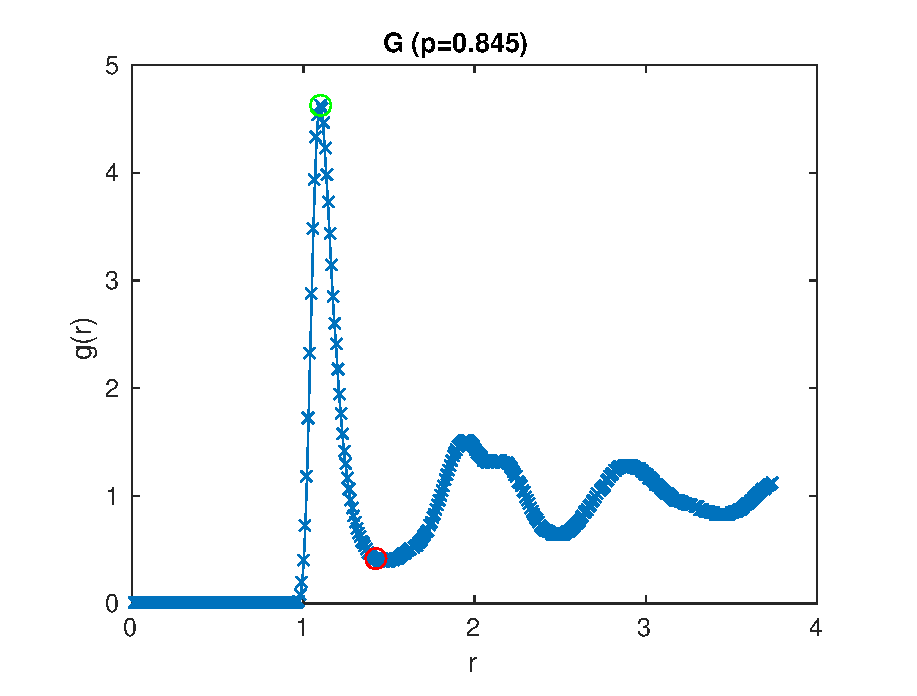
\includegraphics[width=\textwidth]{p2}
\end{figure}
\\
\section{P3}
The actual density in this simulation run was 0.844.
The numerical integration of $g(r)$ across its entire range (0 to 3.75) produces a total particle number of 183.9, in close agreement with the theoretical value of 186.4.
The actual number of particles in the simulation system was 356, in close agreement with the expected number of particles in a 7.5x7.5x7.5 cube (356.06).

\end{document}
